% Chapter 5

\chapter{Perspectives}

\label{Chapter5}

In this last chapter we want to discuss some open problems and approaches to solve them which have not yet been covered within this thesis and might motivate the interested reader for further research.

\section{Applying the cycle detection theorem}

The cycle detection theorem (Theorem \ref{theorem9}) by Kozlov seems to be a key tool to find new cosystoles, but as discussed in Chapter \ref{Chapter2} it is difficult on the one hand to find a large number of cycles on which a given cochain evaluates to \(1\) and on the other hand, once we found such a family of cycles, to determine its hitting number.\\
The first approach might be to develop a theory about hitting numbers for families of cycles, which most likely becomes very challenging, since even for the most obvious family of cycles, namely the boundaries of simplices, a proper generalization of Mantel's theorem (see \cite{7}) has not been discovered yet.\\
An important observation from Chapter \ref{Chapter2} also shows, that it is not sufficient only to study those obvious families of cycles. The family \(\mathcal{T}_{\varphi}\) introduced in Chapter \ref{Chapter2} is obviously the largest possible family of boundaries of simplices doing the job, since by definition it consists of all boundaries of simplices, on which \(\varphi\) evaluates to \(1\). But considering Example \ref{example1b} we see that this family is not always sufficient to determine to cosystolic norm of \(\varphi\) by its hitting number.\\
Nevertheless, even if it is very difficult to determine the hitting number for an arbitrary set of cycles - generally this problem is NP-complete (see \cite{12}) - it might become easier when considering only those families on whose cycles Cheeger cosystoles evaluate to \(1\). The second approach is to search for families of cycles, such that the supports of the cycles in a family are paiswise disjoint, so that we do not have to care about hitting numbers anymore and can just apply Corollary \ref{corollary1}. The disadvantige of this option is, that not all the cosystoles can be determined this way, as an example easily shows. Consider the cochain
\[
\varphi=\left(\{1,2\}+\{3,4\}\right)^*\in C^1(\Delta^{[4]})
\]
(Figure \ref{figure6:Figure 6} shows how the support of this cochain can be imagined), then we can only find a single cycle in \(C_1(\Delta^{[4]})\) satisfying the necessary assumpions, since the support of every second cycle would intersect the support of the first one, but it is easy to see, that we have \(\|\varphi\|_{csy}=2\). Note, that the preceding cosystole is even a Cheeger cosystole. Nevertheless, it might be possible that for every simplex \(\Delta^{[n]}\) and every \(k\geq 1\) there exists a Cheeger cosystole \(\varphi\in C^k(\Delta^{[n]})\), such that we can find a family of pairwise disjoint cycles which satisfies the assumptions of Corollary \ref{corollary1} for \(\varphi\).

\begin{figure}[ht]
\centering
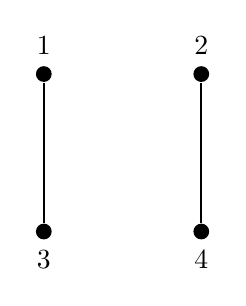
\begin{tikzpicture}[
       thick,
       acteur/.style={
         circle,
         fill=black,
         thick,
         inner sep=2pt,
         minimum size=0.2cm
       }
     ]

       \node (a1) at (0,0) [acteur,label=below:3]{};
       \node (a2) at (0,2)[acteur,label=above:1]{}; 
       \node (a3) at (2,2) [acteur,label=above:2]{}; 
       \node (a4) at (2,0) [acteur,label=below:4]{}; 
  
       \draw (a1) -- (a2); 
       \draw (a3) -- (a4); 

\end{tikzpicture}
  \caption{The support of a $1$-cosystole, which can not be determined using disjoint cycles}
  \label{figure6:Figure 6}
\end{figure}


Finding large families of cycles with pairwise disjoint supports is a problem, that has been approached for example by Peter Keevash (see \cite{11}), who determined the number of vertices \(n\), for which it is possible to partition the uniform \(k\)-skeleton of \(\Delta^{[n]}\), such that every part is the boundary of a (\(k+1\))-simplex.\\
For the case of cut-minimal graphs it might be easier to find large families of edge-disjoint cycles, but since we are not only interested in finding cut-minimal graphs but Cheeger graphs, we still have to handle the challenge of constructing graphs \(G\) by choosing edges in those cycles, such that the number \(T(G)\) becomes as small as possible.

\section{Finding maximal cosystoles of a simplex}

In Theorem \ref{theorem1} we determined the maximum number of edges a cut-minimal graph can have and even discovered the unique (up to isomorphy) shape of such a graph. It always consists of two disjoint as equally large as possible complete graphs. For higher-dimensional cosystoles by now we have no idea about the largest possible norm or the shape of such a largest cosystole. Perhaps, it might be possible to find a lower bound for the maximal norm of a cosystole in general by choosing an adequate family of cycles and using the cycle detection theorem.

\section{The shape of Cheeger graphs if n is a power of 2}

In \cite{1} (Theorem 4.6) Kozlov gave an upper bound for the Cheeger constant \(h_1(\Delta^{[n]})\), if \(n\) is a power of \(2\), using the so called staircase graphs (a certain class of bipartite graphs \(G\) for which the number \(h(G)\) is easy to determine). It is based on the idea to construct Cheeger graphs inductively by adding edges to a graph \(G=([n],\emptyset)\), such that \(G\) stays cut-minimal and the number \(T(G)\) stays as small as possible. Unfortunately, it is not clear if we will always meet a Cheeger graph on this way, since cosystolic complexes have no matroidal structure which would allow to use greedy algorithms to determine the Cheeger cosystoles. Nevertheless, for all the cases when \(n\) is not a power of \(2\) Kozlov showed that it is possible and that this way always leads to a Cheeger graph, which is a staircase graph. So, we conjecture that all Cheeger graphs might be staircase graphs (except for the case \(n=4\)), but even the weaker conjectures, that all Cheeger graphs are bipartite or just triangle-free could not be proven yet. Furthermore, if \(n\) is a power of \(2\), we only know the exact value of the first Cheeger constant for \(n=4\) and \(n=8\) (see \cite{1}, Section 4.2), where it is strictly larger than \(\frac{n}{3}\) and we showed that also for \(n=16\) it has to be strictly larger than \(\frac{n}{3}\) (see Theorem \ref{theoremn=16}). It would be interesting to find it for higher \(n\)'s or at least to figure out, if it might never exactly attain \(\frac{n}{3}\). To approach this challenge, the results from Section \ref{section26} and Chapter \ref{Chapter3} might be helpful as they restrict the shape of Cheeger graphs.

\section{The shape of Cheeger cosystoles in general}

For general Cheeger cosystoles we have a first statement about their shape as Proposition \ref{proposition261} restricting their norm. Maybe one could find more statements of this kind as we already did for Cheeger graphs. Recall, that all Cheeger graphs for \(n\geq 6\) can never be subgraphs of the largest cut-minimal graphs we discovered in Chapter \ref{Chapter3}. One might conjucture, that this property can be generalized to higher dimensional Cheeger cosystoles. Furthermore, one could generalize the concept of staircase graphs by Kozlov (see \cite{1}, Section 3) to general cochains. However, the disadvantage of this approach will be that might become technically difficult and if there are cases where we have \(h_k(\Delta^{[n]})>\frac{n}{k+2}\), we will not be able to determine the exact Cheeger constant using this technique by the same reasons as we had for the Cheeger graphs.

\section{Cheeger constants for other complexes}

Another approach for further research which we totally omitted in this thesis is to study the Cheeger constant for other classes of simplicial or polyhedral complexes. For example in \cite{6} (Theorem 4.3) Kozlov showed that for the \(d\)-dimensional hypercube \(Q_d\) we always have \(h_k(Q_d)=1\). For the more general case of the complex constructed by taking the product of a cell complex and a simplex we only have a rough estimate for the Cheeger constant.

\section{Probabilistic approaches}

Another approach we omitted in this thesis is to use results from probability theory to archieve exact answers to our questions. For example the question, if the cosystolic norm of every cochain can be determined by the cycle detection theorem might be solved in the following way. If we determined the probability of a randomly chosen cochain \(\varphi\in C^k(\Delta^{[n]})\) to be cosystolic and the probability of a ramdomly chosen cochain \(\varphi\in C^k(\Delta^{[n]})\) to provide the smallest hitting set of \(\mathcal{T}_{\varphi}\) as its support, we would get the number of cochains which satisfy each of these properties as expectancy values. If they equaled, we would have proven the conjecture. In fact, we would not even need the exact values of those probabilities. Estimations in the right direction would suffice since we know that any cochain \(\varphi\in C^k(\Delta^{[n]})\) which is not a cosystole can not provide the smallest hitting set for \(\mathcal{T}_{\varphi}\) as its support.